% !TeX root = ../sn.tex
\documentclass[../sn.tex]{subfiles}

\begin{document}
\subsection{What is an IPU?}
In a typical “server optimized” enterprise data center, systems
are designed for use by a single party, that is, the enterprise itself.
However, in a CSP (\textit{Communications Service Providers}) cloud data center, the workload is owned by
the tenant, while the systems themselves are owned by the
Service Provider.

Further, in highly virtualized environments, significant amounts
of server resource are expended processing tasks beyond user
applications, such as hypervisors, container engines, network
and storage functions, security, and vast amounts of network
traffic.

To address this challenge Intel has introduced a new class of
product called the IPU. An IPU is an advanced networking device
with hardened accelerators and Ethernet connectivity that
accelerates and manages infrastructure functions using tightly
coupled, dedicated, programmable cores. An IPU offers full
infrastructure offload and provides an extra layer of security by
serving as a control point of the host for running infrastructure
applications. By using an IPU, the overhead associated with running
infrastructure tasks can be offloaded from the server (Figure 1).
\begin{center}
    \begin{figure}
        \caption{IPU 'disaggregation' in the CSP data center}
        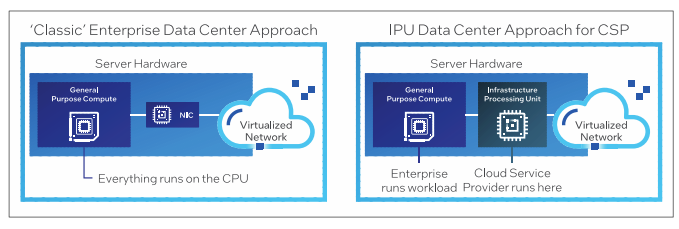
\includegraphics[width=\textwidth]{ipu1.png}
    \end{figure}
\end{center}
In other words, the CSP software runs on the IPU itself, while the
tenant's applications run on the server CPU. This not only frees
up resources on the server, whilst optimizing overall
performance, but provides the CSP with a separate and secure
control point.

It's also important to note the difference between an IPU and
a SmartNIC. A SmartNIC is a programmable network adapter
that can accelerate infrastructure applications, however,
unlike an IPU it does not provide offload capability to run the
entire infrastructure stack and therefore does not give the
service provider an extra layer of security and control,
enforced in hardware.

\subsection{How does an IPU work?}
As data center networking marches forward from 25 GbE, to 50
GbE and into the realm of Terabit Ethernet (100+ GbE), it creates
unprecedented volumes of network traffic. The net result is an
exponential increase in the number of packets transferred per
second putting incremental strain on the capabilities of a traditional
Network Interface Card (NIC).

Additionally, the advent of software-defined networking (SDN)
puts more load onto servers as CPU cores are swallowed up with
virtual switches, load balancing, encryption, deep packet
inspection, and other I/O intensive tasks.
Add into the mix the increasing sophistication of management
software running on servers, and it becomes evident that there
is a genuine need to manage the explosive growth in network
traffic while also offloading “infrastructure” workloads from
server CPUs to enable more resources to be dedicated to
mission-critical application processing.
To put this into context, studies have shown that networking in
highly virtualized environments can consume upwards of 30
percent of the host's CPU cycles \cite{evaleng}.

IPUs combine hardware-based data paths, which can include
FPGAs, with processor cores. This enables infrastructure processing
at the speed of hardware to keep up with increasing network speeds
and the flexibility of software to implement control plane functions.
With the development of its first IPU, Intel has combined onto a
single card an Intel Stratix 10 FPGA, through which a highspeed Ethernet controller and programmable data path is
implemented, along with an Intel Xeon D processor for the
control plane functions.

Blending this capability with the ongoing trend in microservices
development offers a unique opportunity for function-based
infrastructure—achieved through matching optimal hardware
components and common software frameworks to each
application or service. For the CSP, this represents an opportunity to accelerate the
cloud while hosting more services (apps/virtual machines) on a
single machine, leading to improved service delivery and greater
profit potential per server.
\begin{center}
    \begin{figure}
        \centering
        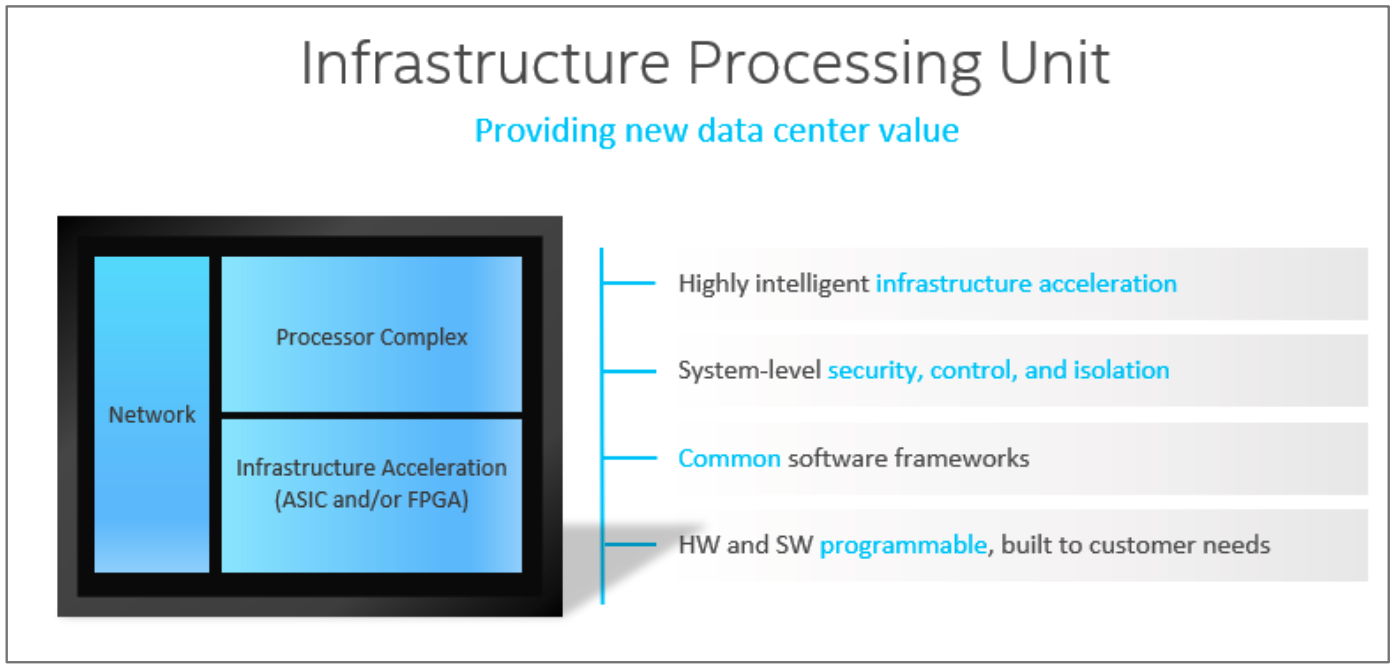
\includegraphics[width=\textwidth]{ipu2.png}
        \caption{IPU conceptual architecture}
    \end{figure}
\end{center}

\end{document}
